\chapter{Pāli Lessons}

These lessons can be included during a Vinaya study period. The material
focues on the language forms used in the Pāṭimokkha, and introduces Pāli
readings from the rules and examples from the daily chants which
bhikkhus have already memorized.

One lesson may take more than one session to study with a group. Someone
familiar with the language may explain the grammar points, while the
others may take turns in solving the exercises.

An \href{https://apps.ankiweb.net/}{Anki Deck} is included to help
memorizing the vocabulary and sentences.

\href{./includes/docs/pali-lessons.pdf}{pali-lessons.pdf}

\href{./includes/docs/pali-lessons.apkg}{pali-lessons.apkg}

\href{./includes/docs/pali-lessons-answerkey.pdf}{pali-lessons-answerkey.pdf}

\href{./includes/docs/pali-lessons.pdf}{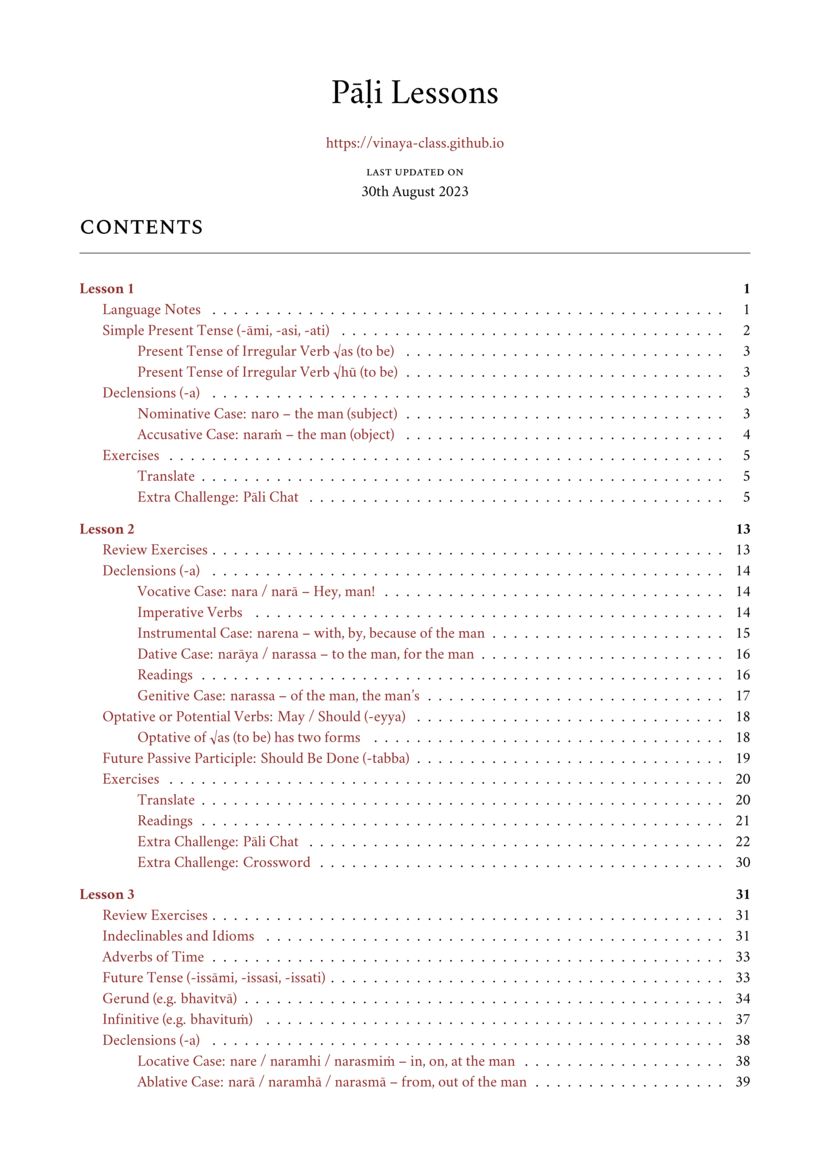
\includegraphics{./includes/docs/pali-lessons-thumb.png}}

